\section{INTRODUCTION}
Recently, aerial robots have attracted a lot of attention and have been studied actively due to their high mobility in three-dimensional environments\cite{Kumar2012}. While there are many applications of aerial robots, such as surveillance\cite{surveillance}, rescue\cite{rescue}, object manipulation and transportation by aerial robots have become an active area of research\cite{lindsey2012}\cite{Mellinger2011}\cite{ZhaoISER2016}\cite{ZhaoICRA2017}\cite{Bernard2009}\cite{Hugh2012}. However, there are still some problems to solve about aerial object transportation. In particular, the endurance of aerial robots is a significant problem. To make the endurance longer, putting bigger batteries can be considered as a solution, but the endurance does not scale linearly with the batteries capacity due to their large weight. Moreover, large weight causes instability of flight. Thus, since it is not easy to make the endurance longer, we must change the point of view. 
\par
To improve the efficiency of aerial object transportation within the limited endurance, we focus on a way that an aerial robot transports multiple objects at the same time. However, it is difficult for conventional aerial robots to transport multiple objects because multiple grippers are necessary to grasp multiple objects, but when the number of objects the aerial robot grasps changes, the center of gravity(CoG) position of the aerial robot changes, resulting that the flight control becomes unstable. Therefore, to achieve this purpose, we focus on multirotor with two-dimensional multilinks\cite{Zhao2016} which possesses the ability to modify the CoG position actively. When picking up an object, the multirotor with multilinks can keep the flight control stable by the aerial transformation by which the CoG position can be modified. In previous works\cite{ZhaoISER2016}\cite{ZhaoICRA2017}\cite{Zhao2016}, quad-rotor with four-links was proposed and extension of the number of links was difficult due to the hardware structure. Therefore, to extend the number of links, a novel structure of multilinks is necessary. Also the communication network must be reliable to achieve stable flight.
\par
The main purpose of this paper is to achieve the construction of the hardware platform of the multirotor with multilinks and multiple objects transportation. Sec. II describes the general approach for the multiple objects transportation. Sec. III clarifies the model of the transformable aerial robot and flight control for aerial transformation. In Sec. IV, we propose the hardware platform which includes the construction of link module and internal communication system. Sec. V explains how to find the optimal form of the multirotor with multilinks based on the flight stability. Finally, we present experimental results in Sec. VI to demonstrate the feasibility of the aerial transformation and multiple object transportation by the multirotor with multilinks. 
\begin{figure}[t]
  \begin{center}
    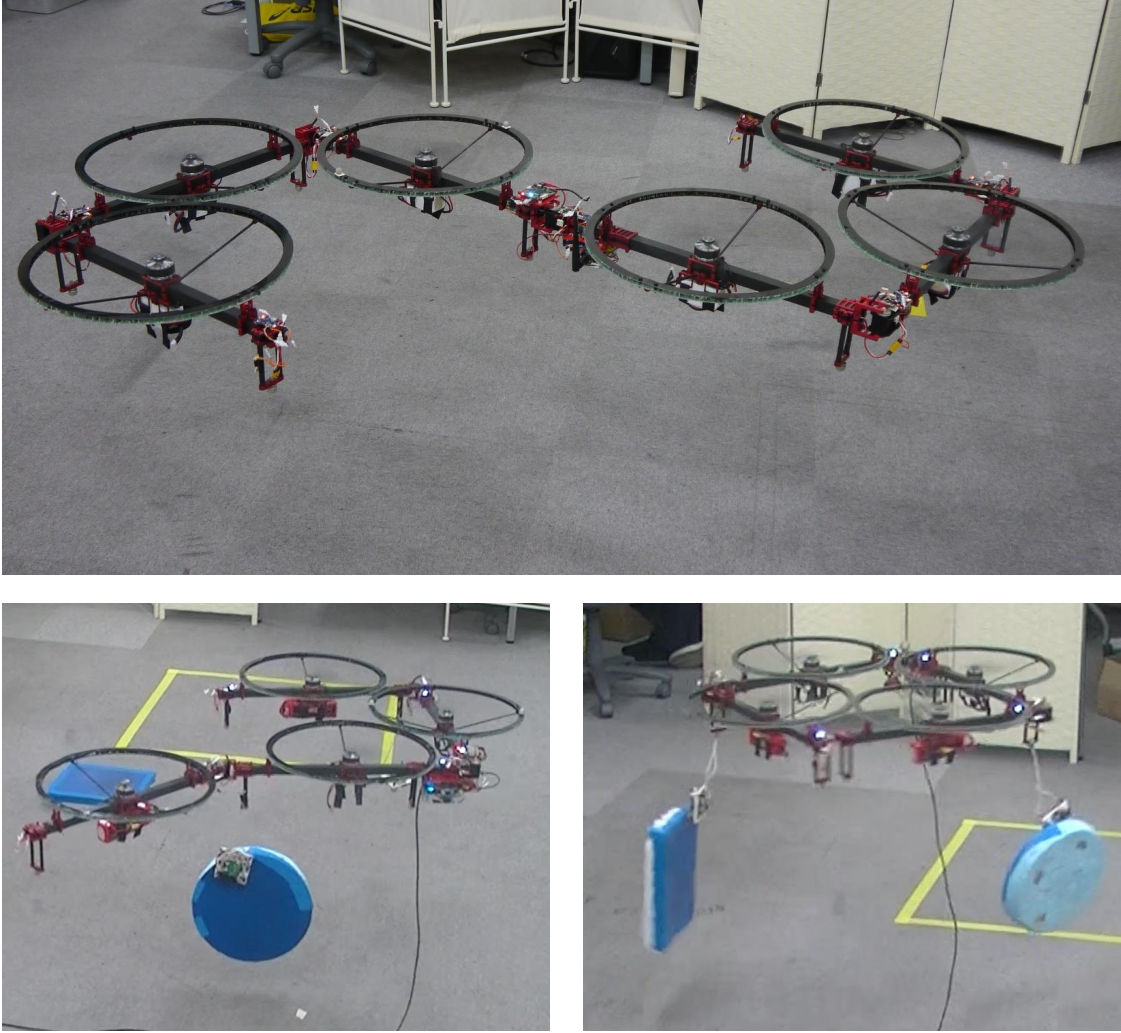
\includegraphics[width=1.0\columnwidth]{figs/object_transportation.pdf}
  \end{center}
  \caption{Upper: the multirotor with multilinks which can transform in the air. Lower left: the aerial robot grasps one object. Lower right: the aerial robot grasps two objects.}
  \label{figure:system}
\end{figure}
